% inspired from http://tex.stackexchange.com/questions/57152/how-to-draw-graphs-in-latex
\documentclass{article}

\usepackage{tikz}
\usetikzlibrary{positioning}
\usetikzlibrary{arrows}

\begin{document}

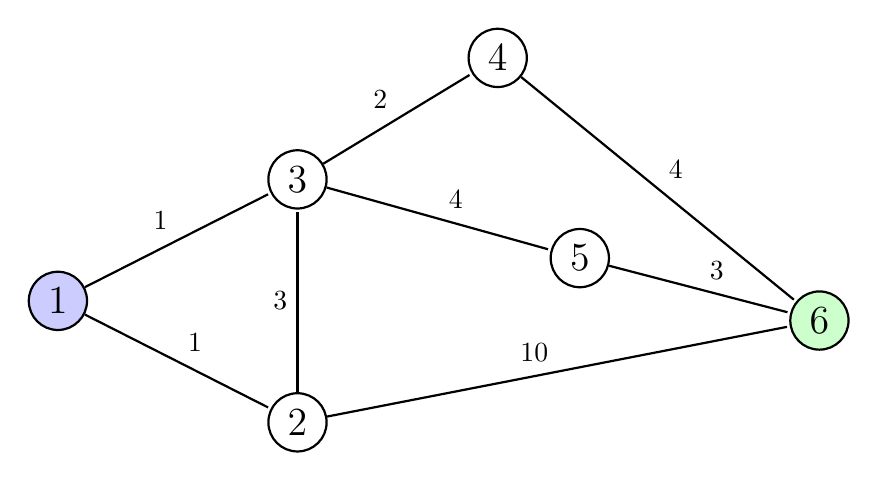
\begin{tikzpicture}[ shorten >=1pt, auto, node distance = 3cm, thick, 
                     node/.style = {circle, draw,
                     font = \sffamily\Large\bfseries}]
\node[node, fill = blue!20] (1) {$1$};
\node[node] (2) [below right = 1cm and 2.5cm of 1]{$2$};
\node[node] (3) [above right = 1cm and 2.5cm of 1]{$3$};
\node[node] (4) [above right = 1cm and 2cm of 3]{$4$};
\node[node] (5) [below right = 2cm and 0.5cm of 4]{$5$};
\node[node, fill = green!20] (6) [below right = 0.25cm and 2.5cm of 5]{$6$};

\path (1) edge node {$1$} (2);
\path (1) edge node {$1$} (3);
\path (2) edge node {$3$} (3);
\path (2) edge node {$10$} (6);
\path (3) edge node {$2$} (4);
\path (3) edge node {$4$} (5);
\path (4) edge node {$4$} (6);
\path (5) edge node {$3$} (6);

\end{tikzpicture}

\end{document}
